\section{Dataset Construction}
\label{sec:data}

No public dataset of EIP-7702 attacks existed when this study began, and existing blockchain-fraud corpora predate the mechanism. We therefore built a dataset directly from the Ethereum ledger. This section describes collection, signer recovery, sampling, outcome-based labelling and the validation of those labels. The design goal throughout was that labels must be derived from information that no detector can observe at its decision time.

\subsection{Collection}
\paragraph{Window} We collected all blocks from the Pectra activation block ($22{,}431{,}084$, 7~May~2025) to block $22{,}863{,}596$ (7~July~2025), a window of $432{,}513$ blocks. The first two months contain the initial adoption of the mechanism by both legitimate wallets and attackers, including the large sweeper campaigns reported by industry~\cite{wintermute2025}.

\paragraph{Authorization scan} Every block was retrieved with full transaction bodies, and every type-\texttt{0x04} transaction was expanded into its authorization tuples. Because the signer of an authorization is not part of the transaction, we recovered it from the secp256k1 signature over the EIP-7702 message digest. To validate recovery, we sampled recovered authorities and compared their current on-chain code with the expected designator $\mathtt{0xef0100}\,\|\,a$; every sampled authority matched. Tuples whose chain identifier was neither $0$ nor $1$, and $21$ tuples with invalid signatures ($0.003\%$), were discarded, as the protocol itself rejects them.

\paragraph{Contract code} For every delegate address we retrieved the deployed bytecode, yielding $661$ distinct delegate contracts.

\paragraph{Account activity} To characterise what happens after a delegation, we collected the value transfers of the accounts involved: every top-level and internal ether transfer that sends value from or to a tracked account, obtained through transaction-trace filtering. Internal transfers are essential, because a sweeper moves funds inside the depositing transaction rather than through a transaction of its own. For each transfer that leaves an authority, we additionally retrieved the sender of the enclosing transaction. This distinguishes outflows initiated by the account owner from outflows triggered by a third party through the delegated code. A second hop collected the activity of candidate attacker sinks---recipients of third-party-triggered outflows---and of the accounts that funded sponsors.

\paragraph{Sampling} Collecting the transfer histories of all $464{,}178$ authorities through public endpoints was infeasible, because the largest sweeper campaigns alone delegated more than $100{,}000$ accounts to a single contract. We applied stratified sampling: every authorization of contracts with at most $1{,}000$ delegators was retained, and $1{,}000$ delegators were drawn uniformly over time for larger contracts. All authorizations made by a sampled authority were kept, so that its delegation history is complete. The working set comprises $165{,}846$ authorizations by $22{,}501$ authorities across all $661$ contracts. Sampling is per contract and uniform in time, so per-contract delegation dynamics are preserved, while the dominance of a handful of mega-campaigns---which would otherwise make any metric an evaluation of those campaigns alone---is reduced.

\subsection{Outcome-based labelling}
A delegation is labelled through its delegate contract. For each contract we aggregate what happened to the accounts that delegated to it, using only outflows from an authority that occur while its delegation is in force and within $24$ hours of it. For each such outflow we record whether it was triggered by a third party (the enclosing transaction was sent by an account other than the authority) and whether its recipient is an externally owned account. A recipient that receives third-party-triggered outflows from at least two distinct authorities of the same contract is a \emph{shared sink}. From these observations we compute, per contract: the number of drained authorities; the drained ratio; the share of drained authorities that drained into shared sinks; the share of all third-party outflow events that terminate in shared sinks; and the share of authorities that continued to initiate their own outflows after delegating (\emph{self-activity}). Table~\ref{tab:labels} lists the decision rules.

\begin{table}[t]
\centering
\caption{Outcome-based contract labelling rules. Contracts meeting neither rule remain unlabelled and are excluded from supervised evaluation.}
\label{tab:labels}
\footnotesize
\setlength{\tabcolsep}{4pt}
\begin{tabular}{p{0.32\columnwidth}p{0.58\columnwidth}}
\toprule
Label & Conditions (all must hold) \\
\midrule
Malicious & $\ge 3$ drained authorities; drained ratio $\ge 0.02$; $\ge 60\%$ of drained authorities drained into shared sinks; $\ge 80\%$ of third-party outflow events end in shared sinks; owner self-activity $\le 20\%$ \\
Benign & $\ge 5$ authorities; drained ratio $\le 0.05$; owner self-activity $\ge 30\%$ \\
\bottomrule
\end{tabular}
\end{table}

The rules encode the operational signature of theft rather than any property a detector uses. A sweeper's victims lose deposits to the same few attacker accounts, the outflows are triggered by whoever sent the deposit rather than by the owner, and owners stop using the account; a benign smart-account implementation shows owners transacting normally and no concentration of value into third-party sinks. Two design choices deserve justification. First, the drained-ratio threshold is deliberately low. A sweeper fires only when funds arrive, and most leaked-key accounts are empty: the largest sweeper in our window, with $968$ delegators in the first week, had drained only $7\%$ of them while concentrating $100\%$ of third-party outflows into shared sinks with $0\%$ owner self-activity. A majority-drained requirement would have labelled it benign. Second, we do not exclude outflows whose recipient equals the transaction sender. In the dominant sweeper pattern the attacker is simultaneously the sponsor, the sender of the draining transaction and its recipient; excluding self-addressed outflows, a natural filter for relayer fees, removed every drain of the largest campaign during development. Relayer fees are instead excluded by the concentration requirement, as they are small and dispersed.

\paragraph{Separation of labels and inputs} Labels depend on outflows that occur \emph{after} each delegation. A detector at decision time $t$ observes only events up to $t$. For evaluation at the moment of authorization, the target's own drains are therefore never visible. Information about \emph{earlier} delegators of the same contract is legitimately visible to a deployed detector and is used by some models; Section~\ref{sec:setup} explains how our evaluation isolates its effect.

\paragraph{Independent cross-check} We matched contracts, their sponsors and their drain sinks against a public scam-address list~\cite{scamsniffer}. No benign contract was linked to a listed address. The list focuses on phishing websites rather than leaked-key sweeping, and none of the malicious contracts' operators appeared on it---an observation that itself illustrates the coverage gap of list-based defences.

\subsection{Statistics}
Table~\ref{tab:stats} summarises the dataset and Fig.~\ref{fig:dataset} characterises it. Delegation volume is dominated by a few campaigns: the delegator distribution per contract is heavy-tailed, and malicious contracts reach tens of thousands of delegators. $67.6\%$ of authorizations are submitted in batches containing more than one authorization, a hallmark of sponsored campaigns. Thefts are almost instantaneous: $67.7\%$ occur in the same block as the authorization and the median delay is zero seconds, because sponsors delegate and invoke the delegated code atomically. This single observation drives a key design requirement: a defence that acts after an authorization is included cannot prevent most thefts.

\begin{table}[t]
\centering
\caption{Dataset statistics (Ethereum, 7 May -- 7 July 2025).}
\label{tab:stats}
\footnotesize
\begin{tabular}{lr}
\toprule
Quantity & Value \\
\midrule
Authorizations (all) & 637{,}846 \\
\quad non-revoking & 634{,}828 \\
Authorities (distinct accounts) & 464{,}178 \\
Sponsors (distinct submitters) & 63{,}951 \\
Delegate contracts & 661 \\
Authorizations in multi-authorization batches & 67.6\% \\
Working set: authorizations / authorities & 165{,}846 / 22{,}501 \\
Temporal graph: nodes / events & 443{,}800 / 4{,}792{,}530 \\
Distinct (authority, contract) targets & 36{,}473 \\
\quad malicious / benign / unlabelled & 11{,}320 / 3{,}201 / 21{,}952 \\
Labelled contracts: malicious / benign & 49 / 11 \\
Code families (all / labelled) & 334 / 41 \\
\quad labelled families: malicious / benign & 32 / 9 \\
Attack campaigns (connected components) & 30 \\
Thefts in the authorization's block & 67.7\% \\
Median authorization-to-theft delay & 0 s \\
\bottomrule
\end{tabular}
\end{table}

\begin{figure}[t]
\centering
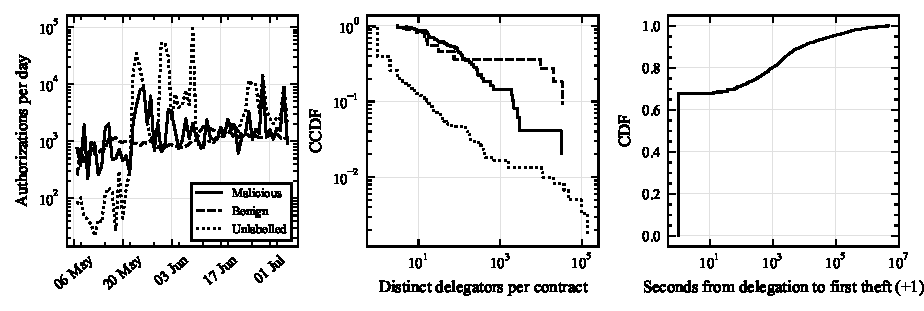
\includegraphics[width=0.4\textwidth]{fig_dataset}
\caption{Dataset characterisation. Left: daily authorizations by contract label (log scale); sweeper campaigns produce bursts of tens of thousands of authorizations per day. Centre: complementary cumulative distribution of distinct delegators per contract; malicious contracts dominate the heavy tail. Right: cumulative distribution of the delay from authorization to first theft; two thirds of thefts occur in the same block.}
\label{fig:dataset}
\end{figure}

\paragraph{Targets} A sweeper often re-authorizes the same victim repeatedly. To prevent near-duplicate examples from appearing on both sides of a split, the prediction target is the first authorization of each (authority, contract) pair, yielding $36{,}473$ targets, of which $14{,}521$ belong to labelled contracts.

\paragraph{Code families} Copy-pasted contracts differ in hard-coded addresses and minor edits, so contract identity is too fine a unit for generalisation tests. We group contracts into \emph{code families} by canonical opcode four-gram Jaccard similarity of at least $0.8$ (Section~\ref{sec:method}), using union-find over exact canonical duplicates first. This yields $334$ families, $41$ of them labelled ($32$ malicious, $9$ benign). The scarcity of benign families---the consequence of requiring at least five delegators and sustained owner activity---is the dataset's principal limitation and recurs in our analysis of learned model combination (Section~\ref{sec:discussion}).

\paragraph{Campaigns} For attribution analysis, malicious delegations are connected when they share a delegate contract, a sponsor or a first drain sink; connected components define $30$ campaigns. Campaign identifiers are used only to score attribution, never as model inputs.
